
\begin{dialog}{前奏曲…}

\begin{quote}
阿基里斯和乌龟来到他们的朋友螃蟹家里,见到了螃蟹的朋友食蚁兽。介绍了一番之后,四个朋友坐下来喝茶。
\end{quote}

\begin{dialogue}

\item[乌龟]老蟹,我们给你带来了一点东西。

\item[螃蟹]真太费心了,你们干嘛这么客气。

\item[乌龟]只是表示一下我们的敬意。阿基,把它拿给老蟹吧。

\item[阿基里斯]好的。老蟹,谨以此表达最美好的祝愿。愿你能喜欢它。

\dnote{(阿基里斯把礼物递给螃蟹,那是个齐整漂亮的小包,方方的,很薄。螃蟹开始拆它。)}

\item[食蚁兽]会是什么呢?

\begin{figure}
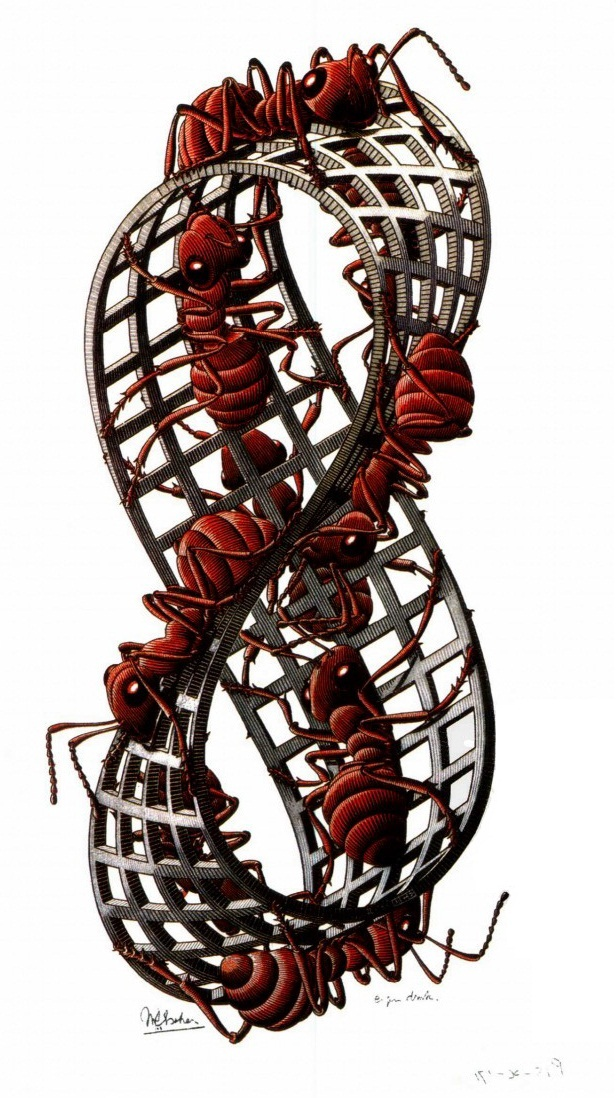
\includegraphics[height=.9\textheight]{img_054.jpg}
\caption[莫比乌斯带II,艾舍尔作。]
  {莫比乌斯带II,艾舍尔作(木刻,1963)。}
\end{figure}

\item[螃蟹]马上就知道了。\dlnote{(拆开之后,拿出了礼物。)}两张唱片!真是太好了!可是没有标签,嗯嗯——龟兄,这又是你的一个“特别礼物”吗?

\item[乌龟]如果你指的是破坏唱机的唱片,那这次不是。不过这唱片的确是特别录制的,全世界独一无二。说实在的,从来还没有人听过呢——当然除了巴赫当时演奏的时候。

\item[螃蟹]巴赫当时演奏的时候?你到底指什么?

\item[阿基里斯]噢,老蟹,等龟兄告诉了你这些唱片到底是怎么回事,你会高兴死的。

\item[乌龟]继续说继续说,阿基,告诉他怎么回事。

\item[阿基里斯]由我来说?这可不是件容易的事!我还是查查我的笔记吧。\dlnote{(取出一张小卡片,清了清嗓子。)}啊哼。你们有兴趣听听数学上一个令人瞩目的新结果吗?你之所以能得到这些唱片,都应归功于这一结果。

\item[螃蟹]我的唱片是来自什么数学结果?其奇怪!好吧,你已经逗起了我的好奇心,我得听个究竟。

\item[阿基里斯]好吧。\dlnote{(停顿了一小会儿,呷了一口茶,然后才开始说起来。)}你们听说过费马那个臭名昭著的“最后定理”吗?

\item[食蚁兽]我说不好……听起来怪熟的,可我想不起来了。

\begin{figure}
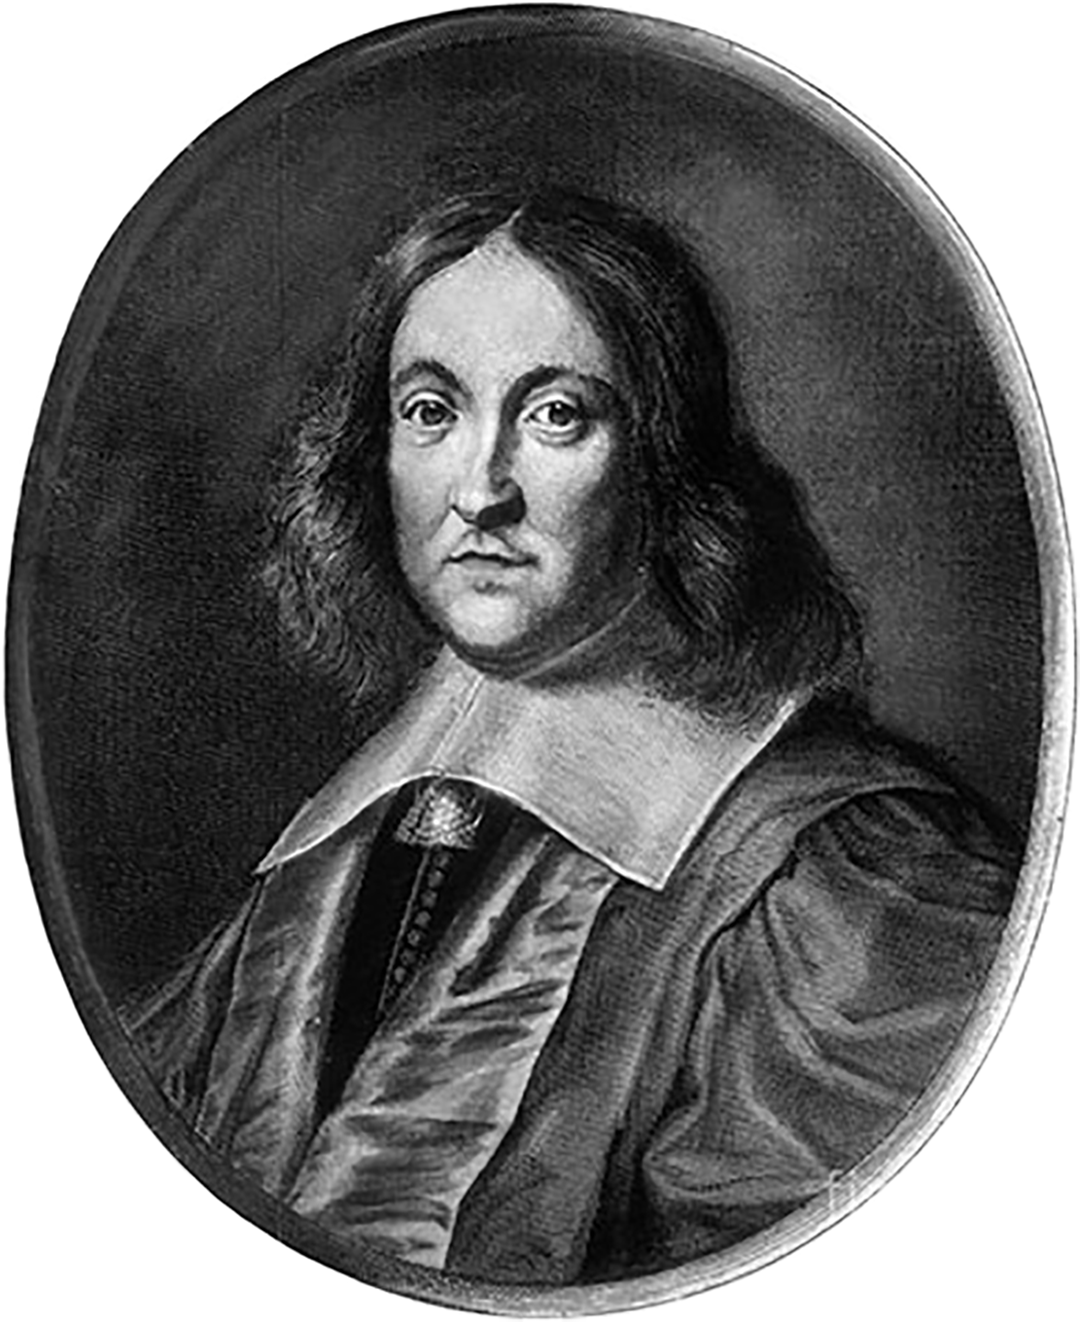
\includegraphics{img_055.png}
\caption[彼埃尔·德·费马。]
  {彼埃尔·德·费马}
\end{figure}

\item[阿基里斯]内容非常简单。彼埃尔·德·费马,这位专业律师、业余数学家,在读一本丢番图的经典教本《算术》时,看到了这样一个方程式:
\[
  a^n+b^n=c^n
\]
他立刻意识到有无穷多个$a$、$b$、$c$能满足这个方程,于是在书的边空上写下了下面这段臭名远扬的批注:
\begin{quote}
方程
\[
  a^n+b^n=c^n
\]
其中$a$、$b$、$c$及$n$取正整数,仅当$n=2$时有解(此时将有无穷多的三元组$a$、$b$、$c$满足这个方程);但$n>2$时没有解。我已找到了一个精彩的证明,可是不凑巧,这里的边空太小了,我无法写下它。
\end{quote}

从三百多年前的那天起,数学家们绞尽脑汁,试图做到:或者证明费马的断言,从而维护费马的名誉——因为由于一些人怀疑他并没有真的找到他所说的那个证明,费马的名声多少有些不佳——或者否定费马的断言,找一个反例:给出四个整数$a$、$b$、$c$和$n$,其中$n>2$,满足那个方程。直到最近,这两个方向上的努力都是失败的。诚然,这个定理已在许多具体的$n$值上被验证是成立的——即那些小于$125000$的$n$值。

\item[食蚁兽]既然没有一个真正的证明,是不是该称之为“猜想”而非“定理”?

\item[阿基里斯]严格说来,你是对的。但习惯上一直这么叫。

\item[螃蟹]有什么人最终解决了这个著名的问题吗?

\item[阿基里斯]你说着了!事实上,正是龟兄解决的,像以往一样,是靠了绝妙的一招。他不仅发现了费马最后定理的证明(因而使“定理”这个名称成为合法的,也保住了费马的名誉),还找到了一个反例,说明那些持怀疑态度的人具有良好的直觉!

\item[螃蟹]我的天!真是个革命性的发现。

\item[食蚁兽]你别让我们悬在这儿啊,到底是些什么神奇的整数满足了费马方程?我尤其感兴趣的是$n$的值。

\item[阿基里斯]噢,坏了!真对不住大家。简直难以相信,我竟然把写着那些值的那张巨大的纸忘在家里了!太可惜了,那张纸大得没法随身携带。我倒真希望我带来了,现在就给你们看看。不过有一件事我确实记得,也许对你们能有帮助——那个$n$的值是不出现在$\uppi$的连分数展开式中的唯一一个正整数。

\item[螃蟹]噢,真遗憾你没把它带到这儿来。不过没什么理由怀疑你的话。

\item[食蚁兽]无所谓,写成十进制的$n$毫无用处。阿基不是刚刚告诉了我们怎么找到它吗。好了,龟兄,在你取得这个划时代的发现之际,请接受我衷心的祝贺!

\item[乌龟]谢谢。可我觉得比结果本身更重要的是它直接导致的实际应用。

\item[螃蟹]我正盼着知道有什么应用呢,因为我一直觉得数论是数学的王后——数学中最纯的分支——数学中没有应用的一个分支!

\item[乌龟]不只你一个人有这种想法。不过说真的,要想给出一个一劳永逸的论断,说明数学中的某一分支——或者甚至某一个定理——什么时候以及怎样在数学之外产生重要影响,那几乎是不可能的。这种事情往往没法预言——我们目前的情况就是这种现象的一个极好例子。

\item[阿基里斯]龟兄那个一箭双雕的结果创造了音响恢复领域中突破性的成果。

\item[食蚁兽]什么是音响恢复?

\item[阿基里斯]这个名称就解释了它的全部内容:从极其复杂的信息中恢复出音响信息。音响恢复的一项典型任务是,当一块石头投入湖水中之后,从湖面上散开的波纹中恢复出石头入水时的声音。

\item[螃蟹]啊唷,那几乎是不可能的呀!

\item[阿基里斯]可能的。这很像一个人的大脑所做的事:当另一个人的声带发出某种声音后,这个人的耳鼓将振动传送到耳涡中的神经纤维,他的大脑就据此恢复出那种声音。

\item[螃蟹]我明白了。可我还是弄不懂数论是从哪儿掺和进来的,或者说这一切和我的新唱片都有什么关系?

\item[阿基里斯]有关系。在音响恢复的数学中,提出了许多与某种丢番图方程解的数目有关的问题。几年来龟兄一直在努力寻求一种方法,能对目前大气里所有分子的运动进行计算,从中恢复出巴赫两百多年前演奏拨弦古钢琴时的声响,

\item[食蚁兽]那肯定不可能!那些声音已经不可挽回地消失了,永远消失了!

\item[阿基里斯]无知的人就是这么想问题……龟兄在这个问题上花了好几年的心血,终于意识到这全都取决于方程
\[
  a^n+b^n=c^n
\]
有多少正整数的解,其中$n>2$。

\item[乌龟]当然,我可以解释到底这个方程是怎么提出来的,不过我敢肯定这会让你们不耐烦。

\item[阿基里斯]结果就是,音响恢复理论预言,巴赫的声音可以从大气中所有分子的运动中恢复出来,条件是或者那个方程至少有一个解——

\item[螃蟹]太棒了!

\item[食蚁兽]妙极了!

\item[乌龟]谁能想得到!

\item[阿基里斯]刚才没说完,我说的是“只要或者存在一个解,或者证明没有解!”于是,龟兄谨慎地开始了工作,从问题的两个方面同时入手。结果是,反例的发现是找出证明的关键组成部分,因此得到一个结果后直接就导致另一个结果。

\item[螃蟹]那怎么会呢?

\item[乌龟]是这样:我指出了费马最后定理的任何一种证明——假如有这么个证明——其结构的组织可以用一个漂亮的公式描述,而这个公式凑巧有赖于某个方程的解的值。我惊异地发现后一个方程原来就是费马方程。这是形式与内容之间关系的一个有趣巧合。所以我找到反例后,要做的不过是从这个数出发构造出那个方程没有解的证明。想想看,出奇的简单。我难以想象为什么以前从未有人发现这个结果。

\item[阿基里斯]由于数学上的这个出乎意料的巨大成功,龟兄因而能实现他梦想已久的音响恢复了。老蟹得到这件礼物标志着所有抽象的工作都已化为可见的现实。

\item[螃蟹]难道这是巴赫演奏他自己的羽管键琴作品的录音?可不要蒙我!

\item[阿基里斯]我很抱歉,这可不是蒙你,这是事实!这两张唱片是一套,录的是约翰·塞巴斯第安·巴赫亲自演奏他的《平均律钢琴曲集》的全部作品。一张唱片是上集,另一张是下集,也就是说,每张唱片都有前奏曲及赋格曲共24首——每个大调及每个小调都有前奏曲及赋格曲各一首。

\item[螃蟹]这珍贵无比的唱片我一定要听听,马上就放,绝对的!哎,我该怎么谢你们二位呢?

\item[乌龟]我们已经很满足了,你为我们准备了这么好的茶。

\dnote{(螃蟹从套中抽出了一张唱片,放了起来。一位羽管键琴演奏家以难及置信的高超技巧进行演奏的乐声充满了屋子,声音的保真度好得难以想象。人们甚至可以听见——或者是想象到?——巴赫一边演奏一边低吟时那轻柔的嗓音……)}

\item[螃蟹]你们谁要看着总谱听吗?我正好有一本《平均律钢琴曲集》,是独一无二的版本,我的一位老师在其中用文字构成了许多复杂的插图,他恰好还是位难得的书法家。

\item[乌龟]能读总谱可太好了。

\dnote{(螃蟹走到他那漂亮的书橱前,打开门,取出两大册谱子。)}

\item[螃蟹]给你,龟兄。我一直没能真正弄懂这个版本中所有那些精美的插图。也许你的礼物会进一步促使我理解它们。

\item[乌龟]我真希望能这样。

\item[食蚁兽]你们注意没有,在这些曲子中前奏曲总是为继后的赋格恰到好处地确定了基调。

\item[螃蟹]是的。虽然很难用语言说清楚,那两个曲子之间的确总是有着某种微妙的关系。即使前奏曲与其赋格没有共同的旋律主题,仍然会有某种两者都具有的无形的抽象特性,把它们紧密地联在一起。

\item[乌龟]前奏曲与赋格之间短暂的休止是极富于戏剧性的——在这里,单音的赋格主题即将奏出,稍后,这个主题与自己交织,形成越来越复杂的奇异优美的和声层次。

\item[阿基里斯]我懂你的意思。有好多前奏曲与赋格我还不太懂,那沉默构成的短暂插曲总让我激动不已,而我总是在那一段间歇里揣度老巴赫下面的意图。比如说,我总是想知道赋格的速度将是什么:快板还是慢板?$6/8$的,还是$4/4$的?三声部的,还是五声部的——或者四声部?然后,第一声部开始了……多么美妙的时刻!

\item[螃蟹]啊,真的,我还记得我年轻时那些逝去的日子,那时候每支新的前奏曲与赋格都使我激动,它们那新奇与优美让我兴奋不已,我常常会感受到不期而至的惊讶。

\item[阿基里斯]现在呢?那些激动都没有了吧?

\item[螃蟹]由于熟悉而消失了。任何激动不都是这样吗?不过在这种熟悉里面包含着深度,算是对消失了的激动的一种补偿。比方说,我发现总有我以前没注意到的东西。

\item[阿基里斯]有一些你以前未曾注意的主题出现?

\item[螃蟹]也许吧——尤其是当它逆转着藏在其他的几个声部中,或者从底层突然涌现出来。另外还有那些了不起的变调,充满了不可思议的奇迹,使人百听不厌,禁不住想知道老巴赫是怎么想出来的。

\item[阿基里斯]最初听到《平均律钢琴曲集》的时候,我有一阵子喜欢得都要痴颠了。那都是过去的事了,现在你说里面还有可期待的,我真是高兴——虽然这也让我感到悲哀,这个阶段对于我来说已是一去不复返了。

\item[螃蟹]噢,你不必担心你那种痴颠会彻底泯灭。年轻时那种痴颠的一个美妙之处就是它总能起死回生,恰恰就在你觉得它终于泯灭了的时候。需要的仅仅是外界恰到好处的触发,

\item[阿基里斯]真的吗?你说具体点好吗?

\item[螃蟹]比如说通过另一个人的耳朵来听,对于这另一个人来说听这支曲子是一次全新的体验——比如说这另一个是你,阿基。兴奋不知怎么传了过来,我就又一次感到激动了。

\item[阿基里斯]这可真有意思。那激动在你身体里休眠了,而你自己却无法从你的潜意识中把它勾出来。

\item[螃蟹]正是这样。在我的大脑结构中,那种激动的潜在的复苏以某种未知的方式“编了码”,我无法随意唤醒它,必须等着偶然的环境来触发。

\item[阿基里斯]我有一个关于赋格的问题,真有点不好意思开口。对我这样一个刚刚起步的赋格听众,也许你们哪位赋格欣赏专家能给我一些帮助……?

\item[乌龟]要是确实能对你有所帮助,我当然愿意提供我这一点点关于赋格的知识。

\item[阿基里斯]谢谢。让我找一个合适的角度来提这个问题。你们对艾舍尔的画《魔带和立方架》熟悉吗?

\begin{figure}
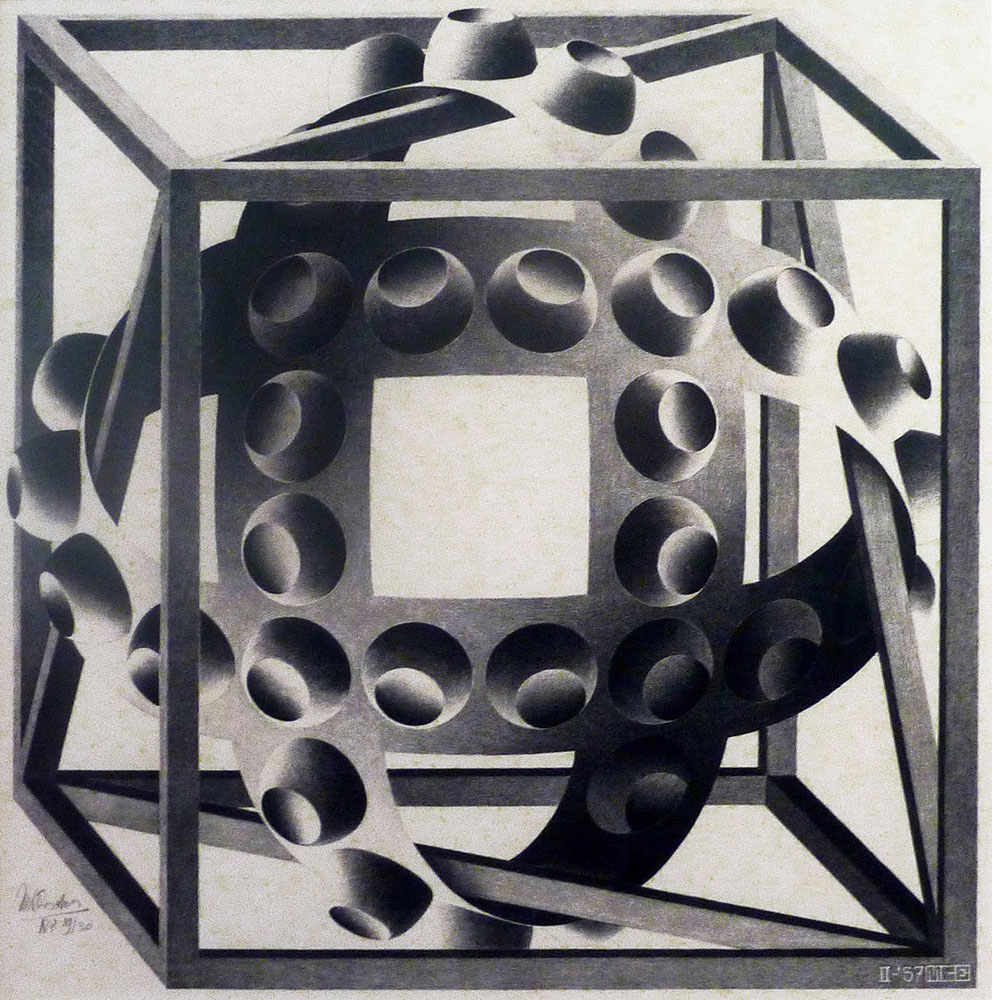
\includegraphics{img_056.jpg}
\caption[魔带和立方架,艾舍尔作。]
  {魔带和立方架,艾舍尔(蚀版画,1957)。}
\end{figure}

\item[乌龟]画的是些环状的带子,上面有小泡一样的东西,你若觉得它们是小包,它们似乎就变成了小坑——反过来也一样,是吗?

\item[阿基里斯]没错。

\item[螃蟹]我记得那幅画。那些小泡泡总是随着你看它们的角度而在凸与凹之间变来变去。没办法把它们同时看成凸的和凹的——人的大脑不知怎么不允许那样。在人们看那些泡泡时,有两种互相排斥的方式。

\item[阿基里斯]就是这样,我似乎发现我听赋格时,也有类似的两种方式。那就是:或者在一段时间里只跟着一个声部,或者,听所有声部合在一起的总体效果,不去从中区分出某个声部。我曾试过两者兼顾,结果非常沮丧,两个方式中的任何一个都会封闭住另一个。我的确没有能力跟着一个声部听下去,同时还能听总体效果。我发现我不经意地在两种方式之间跳来跳去。我并没有要这样,这多少是自发的。

\item[食蚁兽]就像你看那个魔带的时候一样,是吗?

\item[阿基里斯]是的。我想知道的是……是不是我谈起这两个方式,恰恰表明我无疑是个无知的、毫无经验的听众,甚至完全不可能抓住那种超出了我的知识范围的更深的感受方式?

\item[乌龟]不,完全不是。当然我只能说说我自己,我发现我也是在两种方式之间换来换去,虽然并没有下意识地努力控制哪种方式应该占上风。我不知道在座的哪位是否也有类似的体验。螃蟹:当然有。这是个很撩人的现象,这使你觉得那赋格的本质在你周围飘来飘去,你无法全都把握住,因为你不能让自己同时使用两个方式。

\item[食蚁兽]赋格就是这么有趣,它的每个声部自身都是一首乐曲,因而一支赋格可以被当作同时演奏的、建立在同一个主题上的几支不同乐曲的总合。怎么听取决于听众(或他的下意识),或者当作一个整体,或者当作彼此独立并且彼此和谐的几个部分。

\item[阿基里斯]你说那几个部分是“独立的”,这不太准确。它们之间肯定有某种契合,否则把它们放在一起只会是些杂乱无章的声响——这与事实差得太远啦。

\item[食蚁兽]更好的一种说法是:如果你单独听某个声部,你会发现它似乎是自足的。它可以独立存在,这就是为什么我说它是独立的。不过你也是对的,你指出了这些自足的各具意义的部分是秩序井然地彼此溶合在一起的,它们形成一个优美的整体。写出好赋格正是来自这种能力:使听众觉得有几支不同的旋律,每支旋律都好像是由于其自身的美而被写出来的,然而放到一起形成一个总体时,一点也不觉得勉强。我们所遇到的两难现象——即把一支赋格当作一个总体去听与只听它的某个声部——只是一种非常普通的两难现象的特例。许多种从较低层次搭起来的结构都具有这种两难现象。

\item[阿基里斯]噢,真的?你是说我那两种方式会有更一般的表现形式,适用于听赋格之外的情况,是吗?

\item[食蚁兽]绝对正确。

\item[阿基里斯]那怎么会呢。我猜想这与某种交替现象有关,一种把某个东西作为整体感受和作为部分的组合来感受时出现的现象。不过我只在听赋格时遇到过这种现象。

\item[乌龟]噢,天哪,都来瞧啊!我跟着音乐刚翻到这页,就见到这幅极妙的插图,正好对着这首赋格总谱的第一页。

\item[螃蟹]我以前从未见过这幅图,你为什么不让大家都看看?

\dnote{(乌龟把起那本书传给大家。每个人都以自己的特有方式看着那幅图——这个离得远远的,那个凑到近前,每个人都这样或那样地歪着脑袋,困惑不解。最后,又传回到乌龟手里,他全神贯注地看着。)}

\item[阿基里斯]啊,我觉得这支前奏曲马上就要结束了。不知道听了接下来的那支赋格之后,我对下面这个问题是否会有更好的理解:“以什么方式去听赋格是正确的——作为一个整体,还是部分的总和?”

\item[乌龟]仔细听仔细听,会有的!

\end{dialogue}

\begin{quote}
前奏曲结束了。出现了一段静默,然后……
\end{quote}

\begin{flushright}
\lnote{[紧接下段]}
\end{flushright}

\end{dialog}
